\subsection{Сумерки}
\term{Сумерки}~--- часть суток, когда Солнце находится неглубоко под горизонтом.
В зависимости от высоты Солнца под горизонтом различают \imp{гражданские}, \imp{навигационные} и \imp{астрономические} сумерки:\\
\begin{minipage}{0.54\tw}
	\begin{enumerate}
		\item Гражданские~--- от $0^{\circ}$ до $-6^{\circ}$
		\item Навигационные~--- от $-6^{\circ}$ до $-12^{\circ}$
		\item Астрономические~--- от $-12^{\circ}$ до $-18^{\circ}$
	\end{enumerate}
	Когда Солнце опускается ниже $-18^{\circ}$, наступает ночь.
\end{minipage}
\hfill
\begin{minipage}{0.44\tw}
	\centering
	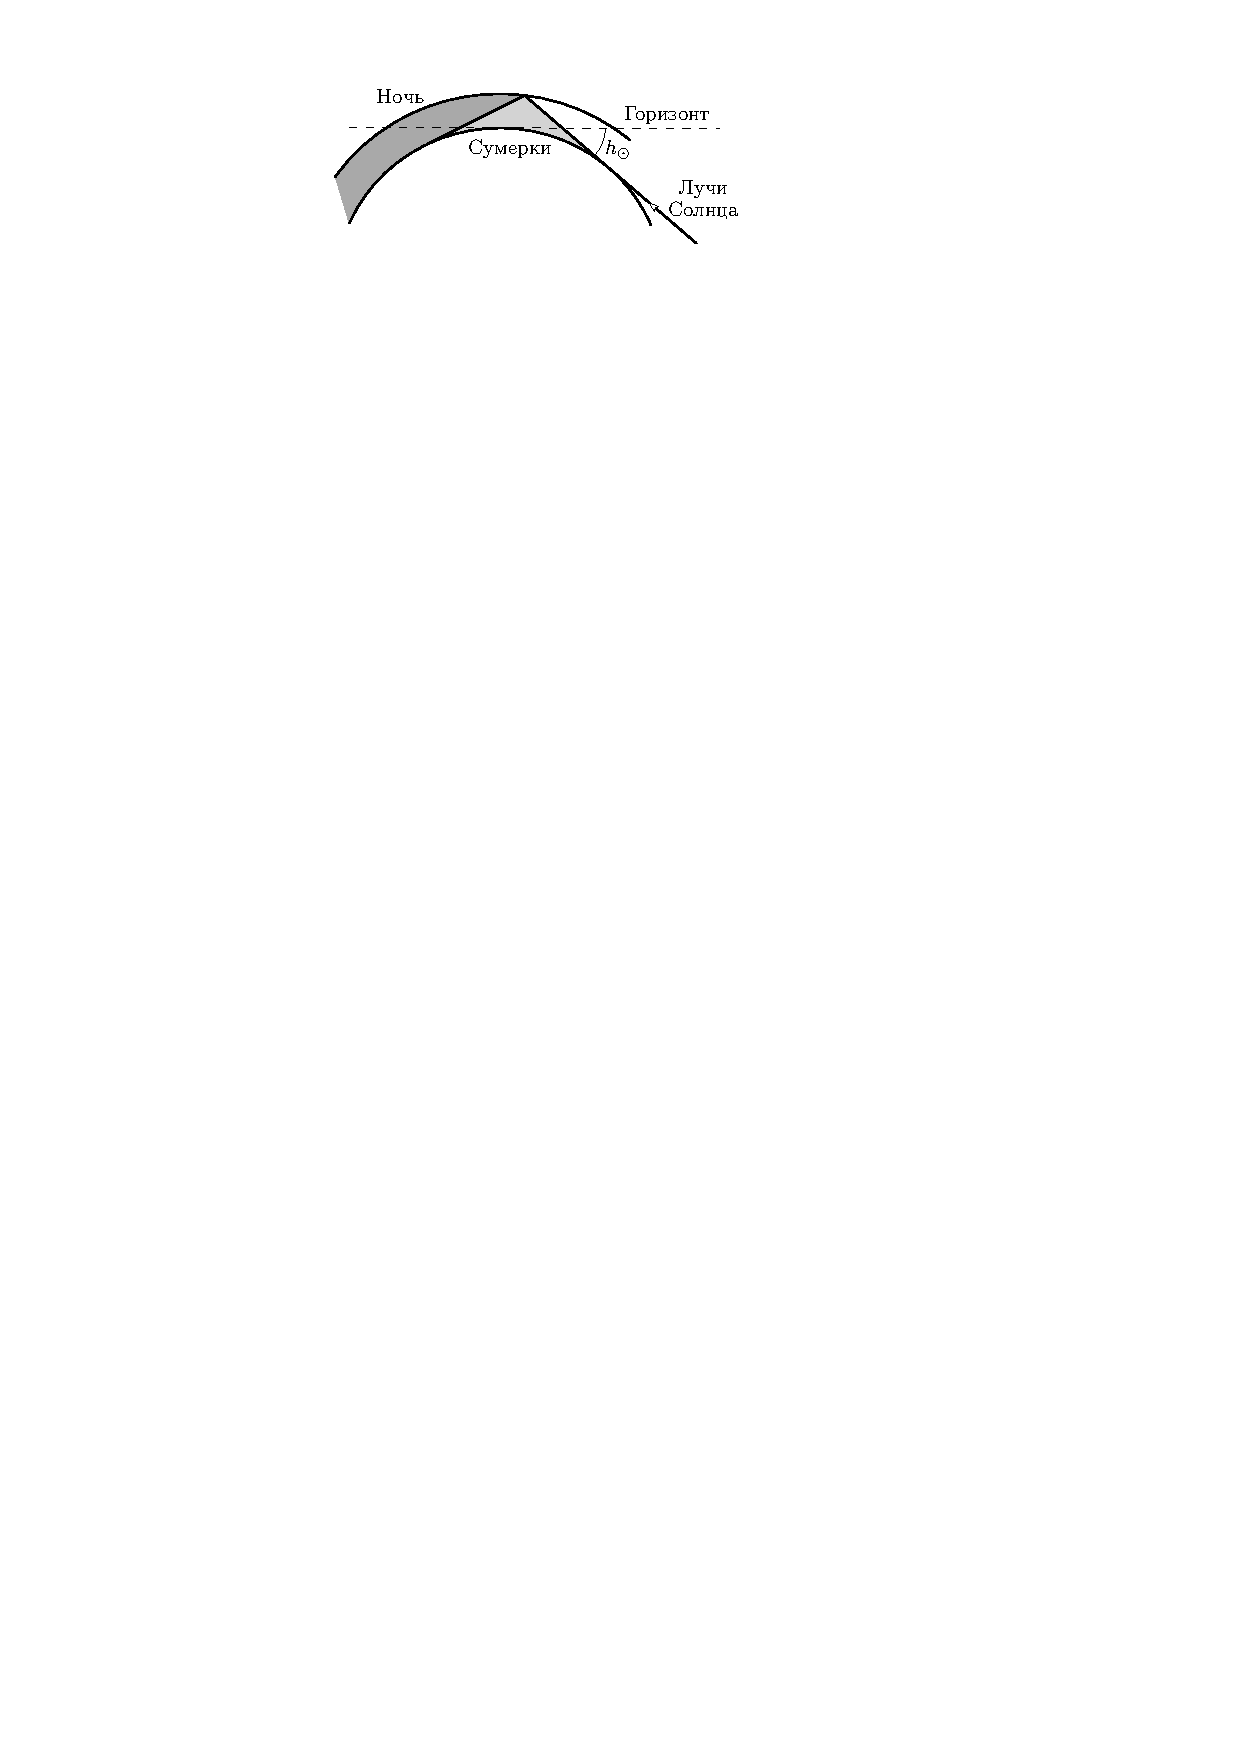
\includegraphics[width=\tw]{spher-astro-dusk.pdf}
	\captionof{figure}{Сумерки}
\end{minipage}
\newpage
